随着项目的发展,在列表文件和源代码中查找内容变得越来越困难。因此,从一开始就保持项目的健康是非常重要的。

想象一下,您需要交付一些重要的、时间敏感的更改,而它们在项目的两个目录中都不适合。现在,需要快速地提交一个清理提交,该提交为文件引入更多的目录和另一层层次结构,以便更改可以有一个合适的位置。或者(更糟糕的是),你决定把它们扔到其他地方,然后手写一张便签,稍后再处理这个问题。

随着时间的推移,这些便签会累积起来,技术债务也会增加,维护代码的成本也会增加。当运行的系统中存在需要快速修复的严重缺陷时,当不熟悉代码库的开发者需要更改时,这就变得非常棘手。

所以,一个好的项目结构意味着什么呢?我们可以从软件开发的其他领域(例如,系统设计)借鉴一些规则。

项目应具备以下特点:

\begin{itemize}
\item 
应该很容易导航和扩展

\item 
应该自包含——例如,特定于项目的文件应该在项目目录中,而不在其他目录中。

\item 
抽象层次结构应该通过可执行文件和二进制文件来表示。
\end{itemize}

没有统一的解决方案,但在网上有很多可用的项目结构模板,我建议采用这个模板,因为它简单,并且易扩展:

\begin{center}
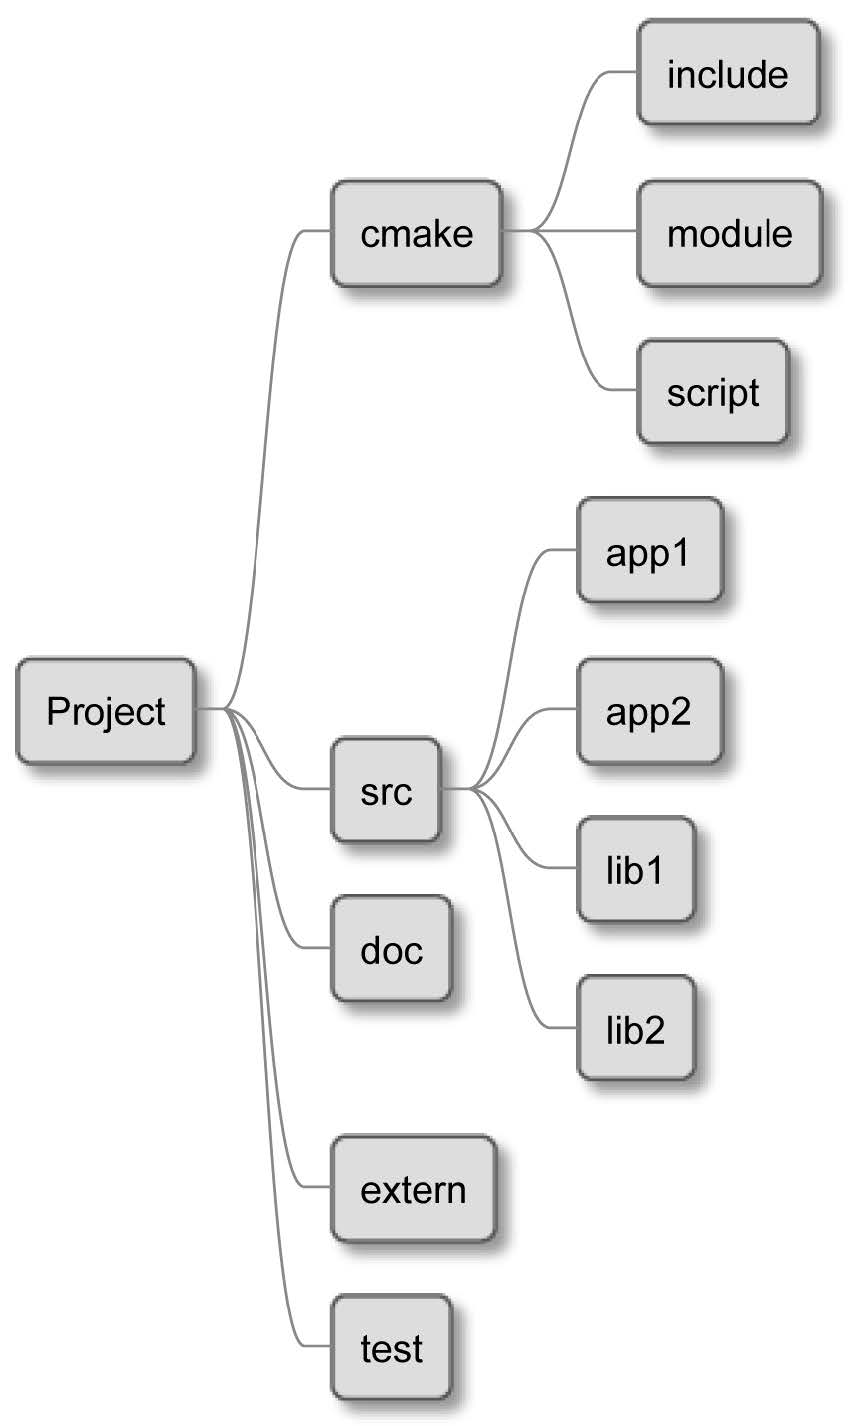
\includegraphics[width=0.5\textwidth]{content/1/chapter3/images/1.jpg}\\
图3.1 项目结构示例
\end{center}

本项目具有以下组件的目录:

\begin{itemize}
\item 
cmake: 包括宏和函数,find\_modules和一次性脚本

\item 
src: 将存储我们的二进制文件和库的源代码

\item 
doc: 用于构建文档

\item 
extern: 从源代码构建的外部项目的配置

\item 
test: 包含自动测试的代码
\end{itemize}

在这个结构中,CMakeLists.txt文件应该存在于以下目录中:顶级项目目录、src、doc、extern和test。主列表文件不应该自己声明任何构建步骤,它应该使用add\_subdirectory()命令来执行嵌套目录中的所有列表文件。反之,若需要的话,可能会把这项工作委派给更深层的层。

\begin{tcolorbox}[colback=blue!5!white,colframe=blue!75!black,title=Note]
一些开发人员建议将可执行文件从库中分离出来,创建两个顶级目录而不是一个:src和lib。CMake对这两个工件一视同仁,在这个级别上的分离并不重要。
\end{tcolorbox}

src目录中拥有多个目录对于更大的项目来说非常方便,若只是构建一个可执行文件或库,可以跳过它们,直接将源文件存储在src中。任何情况下,需要在那里添加一个CMakeLists.txt文件,并执行任何嵌套的列表文件。

这是文件树寻找单个目标的方式:

\begin{center}
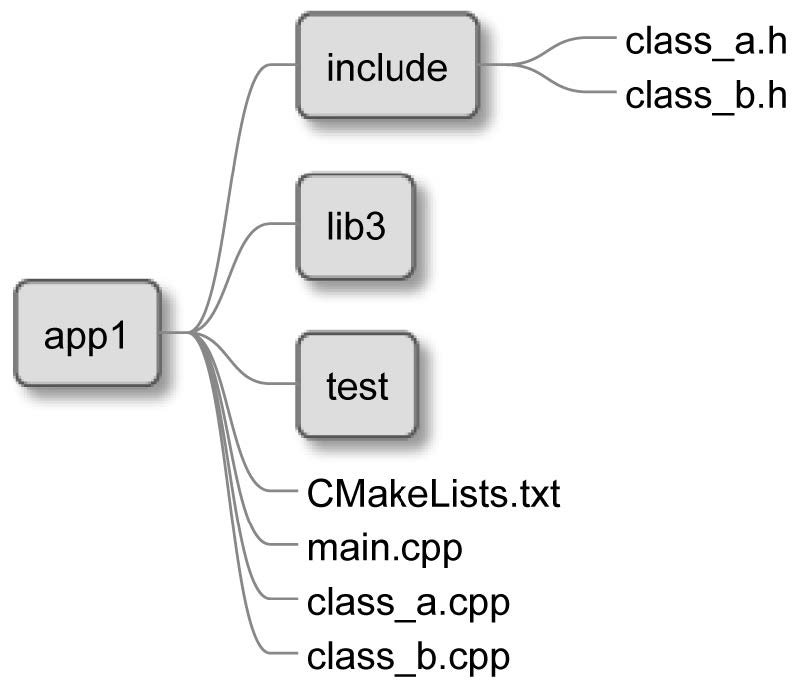
\includegraphics[width=0.5\textwidth]{content/1/chapter3/images/2.jpg}\\
图3.2 可执行文件的目录结构
\end{center}

在app1目录的根目录中看到一个CMakeLists.txt文件——配置关键项目设置并包括来自嵌套目录的所有列表文件。src目录包含另一个CMakeLists.txt文件和.cpp实现文件:两个类和带有可执行文件入口点的主文件。CMakeLists.txt文件应该定义一个使用这些源文件构建可执行文件的目标——将在下一章学习如何做到这一点。

头文件在include目录中——.cpp实现文件使用这些文件来声明来自其他C++编译单元的符号。

我们有一个test目录来存储自动化测试的源码,还有lib3,它只包含一个特定于这个可执行文件的库(在项目的其他地方使用的库或在它之外导出的库应该位于src目录中)。

这种结构非常有表现力,可以对项目进行许多扩展。随着类添加越来越多,可以很容易地将它们分组到库中,以加快编译过程。让我们看看库是什么样子的:

\begin{center}
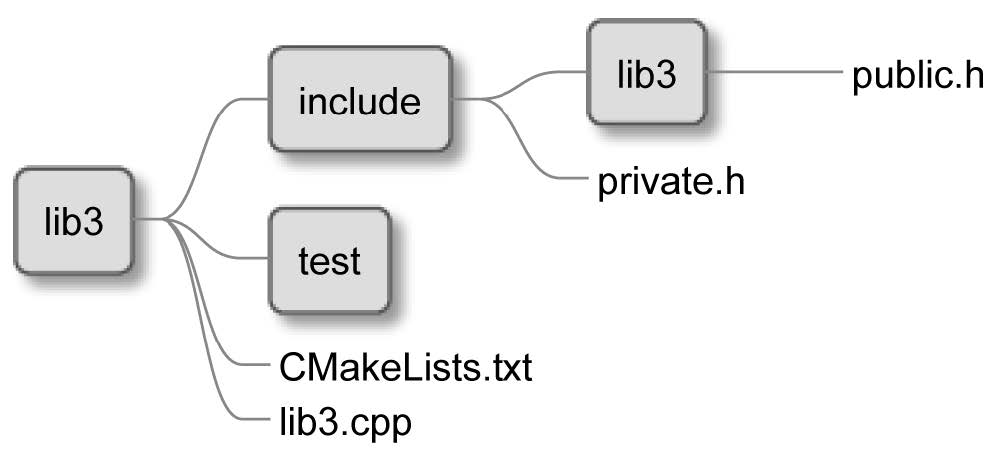
\includegraphics[width=0.6\textwidth]{content/1/chapter3/images/3.jpg}\\
图3.3 库的目录结构
\end{center}

库遵循与可执行文件相同的结构,只有很小的区别:include目录中有一个可选的lib3目录。只有当我们从项目外部使用库时,才会出现这种情况,其提供了其他项目在编译期间将使用的公共头文件。我们将在第5章开始构建自己的库时回到这个主题。

因此,我们已经讨论了如何在目录结构中布局文件。现在,来看看各个CMakeFiles.txt文件是如何组合在一起形成单个项目的,以及其在更大的场景中扮演什么角色。

\begin{center}
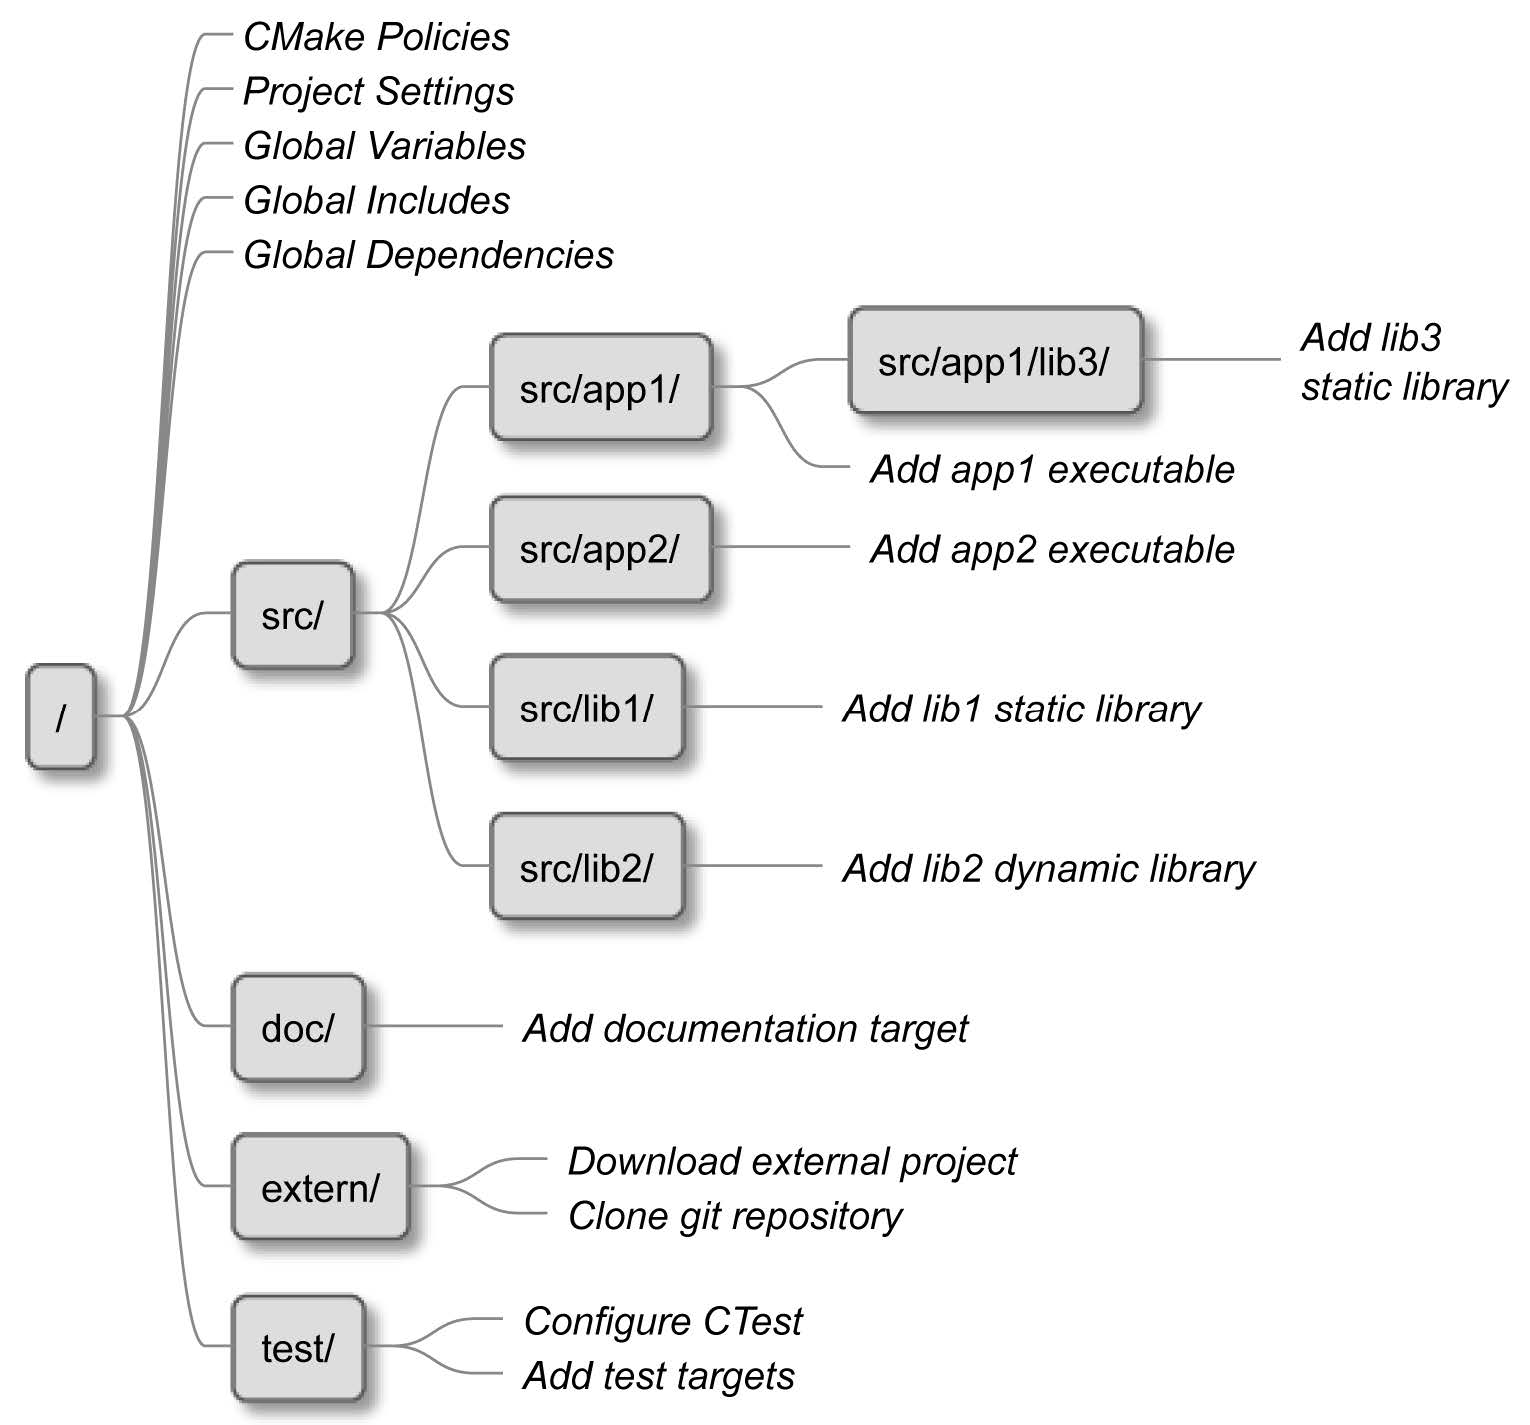
\includegraphics[width=0.8\textwidth]{content/1/chapter3/images/4.jpg}\\
图3.4 CMake如何在单个项目中合并列表文件
\end{center}

图3.4中,每个框表示驻留在给定目录中的CMakeLists.txt列表文件,而文本中的标签表示每个文件执行的操作(从上到下)。让我们再从CMake的角度来分析一下这个项目:

\begin{enumerate}
\item 
执行从项目的根开始——从源码树中的列表文件开始。该文件将使用适当的策略设置最低要求的CMake版本,设置项目名称、支持的语言、全局变量,并包括来自CMake目录的文件,以便它们的内容全局可用。

\item 
下一步是通过使用add\_subdirectory(src bin)指令进入src目录的范围(将编译好的工件放在<binary\_tree>/bin,而不是<binary\_tree>/src)。

\item 
CMake读取src/CMakeLists.txt文件,发现其唯一用途是添加四个嵌套子目录:app1、app2、lib1和lib2。

\item 
CMake进入app1的变量作用域,了解另一个嵌套库lib3,它有自己的CMakeLists.txt文件;然后输入lib3的作用域。

\item 
lib3库添加了一个具有相同名称的静态库目标。CMake返回app1的父范围。

\item 
app1子目录添加了一个依赖于lib3的可执行文件。CMake返回src的父范围。

\item 
CMake将继续进入剩下的嵌套作用域并执行它们的列表文件,直到完成所有add\_subdirectory()调用。

\item 
CMake返回到顶级作用域并执行剩下的三个指令:add\_subdirectory(doc)、add\_subdirectory(extern)和add\_subdirectory(test)。CMake每次都进入新的作用域,并从适当的列表文件执行指令。

\item 
收集所有的目标并检查其正确性。CMake现在拥有生成构建系统所需的所有信息。
\end{enumerate}

前面的步骤的发生顺序与我们在列表文件中写入命令的顺序完全一致。有时这很重要,而另一些时候则不是那么重要。我们将在下一章深入探讨。

那么,什么时候是创建目录以包含项目的所有元素的最佳时间呢?应该从一开始就做正确的事情——创建未来需要的所有东西,并保持目录为空——还是等到我们真正有了需要归入自己类别的文件?这是一种选择——可以遵循极限编程规则YAGNI(不需要它),或者可以尝试让项目具有前瞻性,为接纳新开发人员的到来奠定良好的基础。

试着在这些方法之间取得良好的平衡——若怀疑项目有一天可能需要一个extern目录,那么就添加它(可能需要创建一个空的.keep文件来将目录检入存储库)。为了帮助其他人知道在哪里放置他们的外部依赖项,创建一个自述文件,并为未来将走上这条路的缺乏经验的程序员铺平道路。您可能已经注意到:开发人员不愿意创建目录,特别是在项目的根目录中。若提供一个好的项目结构,人们会倾向于遵循它。

有些项目可以在几乎所有的环境中构建,而另一些项目则对其细节非常挑剔。顶层列表文件是评估如何进行项目的最佳位置,这取决于可用的内容。





